\documentclass[11pt,a4paper]{article}

\usepackage[utf8]{inputenc}
\usepackage[T1]{fontenc}
\usepackage[french,provide=*]{babel}
\usepackage[a4paper,top=2.1cm,bottom=2.4cm,left=2.0cm,right=2.0cm,headheight=18pt]{geometry}
\usepackage{xcolor}
\usepackage{graphicx}
\usepackage{booktabs}
\usepackage{array}
\usepackage{enumitem}
\usepackage{tikz}
\usetikzlibrary{arrows.meta,positioning,shadows.blur}
\usepackage{listings}
\usepackage[most]{tcolorbox}
\usepackage{titlesec}
\usepackage{fancyhdr}
\usepackage[hidelinks]{hyperref}

\definecolor{ink}{RGB}{27,31,42}
\definecolor{paper}{RGB}{252,249,242}
\definecolor{oxide}{RGB}{146,54,44}
\definecolor{lagoon}{RGB}{0,104,117}
\definecolor{sage}{RGB}{225,238,230}
\definecolor{sand}{RGB}{247,232,199}
\definecolor{codeback}{RGB}{18,24,38}
\definecolor{codeframe}{RGB}{0,104,117}
\definecolor{outback}{RGB}{248,245,236}
\definecolor{outframe}{RGB}{183,143,86}
\definecolor{muted}{RGB}{105,113,126}

\pagecolor{paper}
\color{ink}

\pagestyle{fancy}
\fancyhf{}
\fancyhead[L]{\small\textcolor{lagoon}{TP Cryptographie}}
\fancyhead[R]{\small\textcolor{oxide}{Certificats, révocation et HSM}}
\fancyfoot[L]{\small\textcolor{muted}{Baptiste PAQUERIAUD}}
\fancyfoot[R]{\small\thepage}
\renewcommand{\headrulewidth}{0pt}
\renewcommand{\footrulewidth}{0.3pt}

\titleformat{\section}{\Large\bfseries\color{oxide}}{\thesection}{0.7em}{}
\titleformat{\subsection}{\large\bfseries\color{lagoon}}{\thesubsection}{0.7em}{}
\titleformat{\subsubsection}{\normalsize\bfseries\color{ink}}{\thesubsubsection}{0.7em}{}
\titlespacing*{\section}{0pt}{1.6em}{0.8em}
\titlespacing*{\subsection}{0pt}{1.2em}{0.5em}

\lstdefinestyle{shellcmd}{
  backgroundcolor=\color{codeback},
  basicstyle=\ttfamily\footnotesize\color{white},
  breaklines=true,
  breakatwhitespace=false,
  postbreak=\mbox{\textcolor{sand}{$\hookrightarrow$}\space},
  columns=fullflexible,
  keepspaces=true,
  showstringspaces=false,
  frame=leftline,
  framesep=7pt,
  framerule=3pt,
  rulecolor=\color{codeframe},
  xleftmargin=8pt,
  xrightmargin=4pt,
  aboveskip=7pt,
  belowskip=7pt
}

\lstdefinestyle{result}{
  backgroundcolor=\color{outback},
  basicstyle=\ttfamily\scriptsize\color{ink},
  breaklines=true,
  breakatwhitespace=false,
  postbreak=\mbox{\textcolor{muted}{$\hookrightarrow$}\space},
  columns=fullflexible,
  keepspaces=true,
  showstringspaces=false,
  frame=single,
  framesep=6pt,
  rulecolor=\color{outframe},
  xleftmargin=4pt,
  xrightmargin=4pt,
  aboveskip=7pt,
  belowskip=7pt
}

\lstdefinestyle{config}{
  backgroundcolor=\color{sage},
  basicstyle=\ttfamily\scriptsize\color{ink},
  breaklines=true,
  columns=fullflexible,
  keepspaces=true,
  showstringspaces=false,
  frame=single,
  framesep=6pt,
  rulecolor=\color{lagoon!60!black},
  commentstyle=\color{oxide}\itshape,
  morecomment=[l]{\#}
}

\newtcolorbox{answerbox}[1][]{
  colback=sage,
  colframe=lagoon,
  coltitle=white,
  title=Réponse synthétique,
  fonttitle=\bfseries,
  arc=1mm,
  boxrule=0.9pt,
  left=7pt,
  right=7pt,
  top=5pt,
  bottom=5pt,
  #1
}

\newtcolorbox{warningbox}[1][]{
  colback=sand,
  colframe=oxide,
  coltitle=white,
  title=Point à compléter ou à exécuter hors Linux,
  fonttitle=\bfseries,
  arc=1mm,
  boxrule=0.9pt,
  left=7pt,
  right=7pt,
  top=5pt,
  bottom=5pt,
  #1
}

\newtcolorbox{remarkbox}[1][]{
  colback=white,
  colframe=muted,
  coltitle=white,
  title=Observation,
  fonttitle=\bfseries,
  arc=1mm,
  boxrule=0.7pt,
  left=7pt,
  right=7pt,
  top=5pt,
  bottom=5pt,
  #1
}

\newcommand{\tri}{\texttt{APV}}
\newcommand{\file}[1]{\texttt{\detokenize{#1}}}
\newcommand{\codeinline}[1]{\colorbox{sand}{\texttt{\detokenize{#1}}}}

\begin{document}

\begin{titlepage}
\begin{tikzpicture}[remember picture,overlay]
  \fill[lagoon] (current page.north west) rectangle ([yshift=-7.2cm]current page.north east);
  \fill[oxide] ([xshift=-3cm,yshift=-9.5cm]current page.north east) circle (4.2cm);
  \fill[sand] ([xshift=1.2cm,yshift=-23cm]current page.north west) circle (5.3cm);
\end{tikzpicture}
\vspace*{1.2cm}
\begin{flushleft}
  {\color{white}\Large IMT Mines Alès}\\[0.4cm]
  {\color{white}\Huge\bfseries Rapport de TP}\\[0.35cm]
  {\color{white}\LARGE Cryptographie et cycle de vie des certificats}\\[1.2cm]
  {\color{black}\large Analyse X.509, PKI OpenSSL, révocation, S/MIME, certification croisée et SoftHSM2}\\[0.8cm]
  {\color{black}\Large Baptiste PAQUERIAUD}
\end{flushleft}
\vfill
\begin{flushright}
  \begin{tcolorbox}[colback=white,colframe=lagoon,width=0.62\linewidth,arc=1mm,boxrule=1pt]
  \textbf{23 juin 2026}\par
  Réalisé sous Arch Linux
  \end{tcolorbox}
\end{flushright}
\end{titlepage}

\tableofcontents
\newpage

\section{Introduction}

\subsection{Objectifs}
Le TP suit trois axes : l'étude de certificats publics, la création d'une infrastructure de certification OpenSSL, puis l'utilisation d'une racine dont la clé privée reste dans SoftHSM2.

\begin{itemize}[leftmargin=1.4em]
  \item \textbf{Certificats existants :} récupération du certificat TLS de \url{https://cyber.gouv.fr/}, analyse de la chaîne, des extensions, des CRL et de l'OCSP.
  \item \textbf{PKI locale :} construction de deux branches, RSA et ECDSA, avec AC racines, AC subordonnées, entités finales, révocation et certification croisée.
  \item \textbf{HSM virtuel :} création d'une racine OpenSSL adossée à SoftHSM2, sans export de clé privée, puis préparation du lien avec une AC subordonnée ADCS.
\end{itemize}

\subsection{Paramètres cryptographiques retenus}
Les choix suivent les contraintes indiquées dans le sujet et les recommandations ANSSI : RSA au moins 2048 bits, courbes elliptiques au moins 256 bits et SHA-2. Les valeurs techniques sont reprises sans modification.

\begin{center}
\renewcommand{\arraystretch}{1.25}
\begin{tabular}{>{\raggedright\arraybackslash}p{4.5cm} l l l}
\toprule
\textbf{Composant} & \textbf{Algorithme} & \textbf{Taille ou courbe} & \textbf{Hachage}\\
\midrule
\file{RSA_Root_CA_APV} & RSA & 4096 bits & SHA-256\\
\file{Sub_RSA_CA_1_APV} & RSA & 3072 bits & SHA-256\\
\file{EC_Root_CA_APV} & ECDSA & secp384r1 (P-384) & SHA-256\\
\file{Sub_EC_CA_1_APV} & ECDSA & secp384r1 (P-384) & SHA-256\\
Entité finale RSA & RSA & 3072 bits & SHA-256\\
Entité finale EC & ECDSA & prime256v1 (P-256) & SHA-256\\
Racine HSM & RSA & 4096 bits & SHA-256\\
\bottomrule
\end{tabular}
\end{center}

\subsection{Durées et nommage}
\begin{center}
\renewcommand{\arraystretch}{1.18}
\begin{tabular}{l l l}
\toprule
\textbf{Objet} & \textbf{Durée} & \textbf{Paramètre}\\
\midrule
AC racines & 15 ans & \file{5479} jours\\
AC subordonnées & 10 ans & \file{3653} jours\\
Entités finales & 1 an & \file{365} jours\\
CRL / ARL & 1 mois & \file{default_crl_days = 30}\\
Racine HSM & 10 ans & \file{3653} jours\\
AC subordonnée ADCS & 5 ans & \file{1825} jours\\
\bottomrule
\end{tabular}
\end{center}

Le DN commun est \file{C=FR, O=TP IMT Mines Ales, OU=PKI APV}; le \file{CN} porte ensuite le nom de l'entité.

\newpage

\section{Analyse de certificats publics}

\subsection{Récupération et protocole observé}
La connexion HTTPS observée repose sur TLS. La trace OpenSSL indique \file{TLSv1.3}; SSL ne correspond qu'à la dénomination historique.

\begin{lstlisting}[style=shellcmd]
openssl s_client -connect cyber.gouv.fr:443 -servername cyber.gouv.fr -showcerts \
  2>/dev/null </dev/null > cyber.gouv.fr.chain.txt
awk '/BEGIN CERTIFICATE/{c++} END{print c}' cyber.gouv.fr.chain.txt
openssl s_client -connect cyber.gouv.fr:443 -servername cyber.gouv.fr 2>/dev/null </dev/null \
  | openssl x509 -out cyber.gouv.fr.pem
\end{lstlisting}

\begin{lstlisting}[style=result]
2
\end{lstlisting}

\subsection{Chaîne TLS et rôle des autorités}
\begin{answerbox}
La chaîne envoyée par \file{openssl s_client} contient \textbf{2 certificats} : le certificat serveur \file{cyber.gouv.fr} et le certificat subordonné \file{GandiCert}. La racine \file{DigiCert Global Root G2} n'est pas transmise par le serveur, car elle est attendue dans le magasin de confiance du client. L'AC qui émet directement le certificat serveur est \file{C=FR, O=Gandi SAS, CN=GandiCert}. La clé publique du site est une clé \textbf{RSA 4096 bits}.
\end{answerbox}

\subsection{Contenu du certificat feuille}
\begin{lstlisting}[style=shellcmd]
openssl x509 -in cyber.gouv.fr.pem -noout -text > cyber.gouv.fr.x509.txt
\end{lstlisting}

Le certificat est un X.509 v3 d'entité finale pour serveur TLS. Le sujet contient \file{CN=cyber.gouv.fr}; les SAN listés sont \file{DNS:cyber.gouv.fr}, \file{DNS:ssi.gouv.fr}, \file{DNS:www.ssi.gouv.fr} et \file{DNS:www.cyber.gouv.fr}. Les usages étendus se limitent à \file{TLS Web Server Authentication} et les contraintes de base indiquent \file{CA:FALSE}.

\begin{answerbox}
Il ne peut pas signer d'autres certificats : \file{Basic Constraints: CA:FALSE} et le \file{Key Usage} ne contient pas \file{keyCertSign}. Il ne peut pas non plus être utilisé comme certificat S/MIME, car \file{E-mail Protection} / \file{emailProtection} n'apparaît pas dans l'Extended Key Usage.
\end{answerbox}

Les points de distribution CRL présents dans le certificat sont les suivants.

\begin{lstlisting}[style=result]
http://crl3.digicert.com/GandiCert.crl
http://crl4.digicert.com/GandiCert.crl
\end{lstlisting}

Le numéro de série est affiché en hexadécimal par OpenSSL; sa conversion décimale est conservée ci-dessous.

\begin{lstlisting}[style=result]
Serial hex avec separateurs : 05:7e:1f:dd:c4:8e:7a:07:80:64:3a:be:eb:cc:52:a5
Serial hex normalise       : 057E1FDDC48E7A0780643ABEEBCC52A5
Serial decimal             : 7301015708052902158374241928634716837
\end{lstlisting}

Affichage de la clé publique :

\begin{lstlisting}[style=shellcmd]
openssl x509 -in cyber.gouv.fr.pem -pubkey -noout
\end{lstlisting}

\begin{lstlisting}[style=result]
Public Key Algorithm: rsaEncryption
Public-Key: (4096 bit)
Exponent: 65537 (0x10001)
\end{lstlisting}

La clé privée ne peut pas être extraite d'un certificat public. Le certificat contient la clé publique, des métadonnées, des extensions et une signature, jamais le secret du serveur.

\subsection{Contrôle par CRL}
\begin{lstlisting}[style=shellcmd]
wget -O GandiCert.crl http://crl3.digicert.com/GandiCert.crl
openssl crl -inform DER -in GandiCert.crl -text -noout > crl.txt
rg "057E1FDDC48E7A0780643ABEEBCC52A5|05:7E:1F:DD:C4:8E:7A:07:80:64:3A:BE:EB:CC:52:A5" crl.txt
\end{lstlisting}

La CRL consultée a les bornes temporelles suivantes.

\begin{lstlisting}[style=result]
Last Update: Jun 22 12:45:56 2026 GMT
Next Update: Jun 29 12:45:56 2026 GMT
\end{lstlisting}

Sa validité est donc de \textbf{7 jours}. Les premières entrées de \file{crl.txt} affichent principalement numéro de série et date de révocation; des \file{X509v3 CRL Reason Code} existent plus loin mais ne sont pas systématiques au début du fichier. Pour vérifier que la CRL est la bonne, on compare son \file{Issuer} à \file{C=FR, O=Gandi SAS, CN=GandiCert}, on vérifie que l'URL provient des points de distribution, puis on valide la signature avec le certificat de l'AC. La recherche du numéro de série \file{057E1FDDC48E7A0780643ABEEBCC52A5} ne renvoie pas de correspondance : le certificat n'est pas listé comme révoqué dans cette CRL.

\subsection{Certificat révoqué et navigateurs}
Les deux captures disponibles montrent le rejet du site \url{https://revoked-rsa-dv.ssl.com/} par Chrome/Chromium et Firefox.

\begin{figure}[htbp]
  \centering
  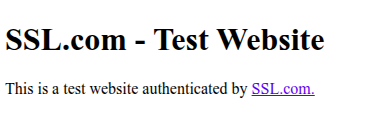
\includegraphics[width=0.48\linewidth]{figures/revoked_rsa_chrome.png}\hfill
  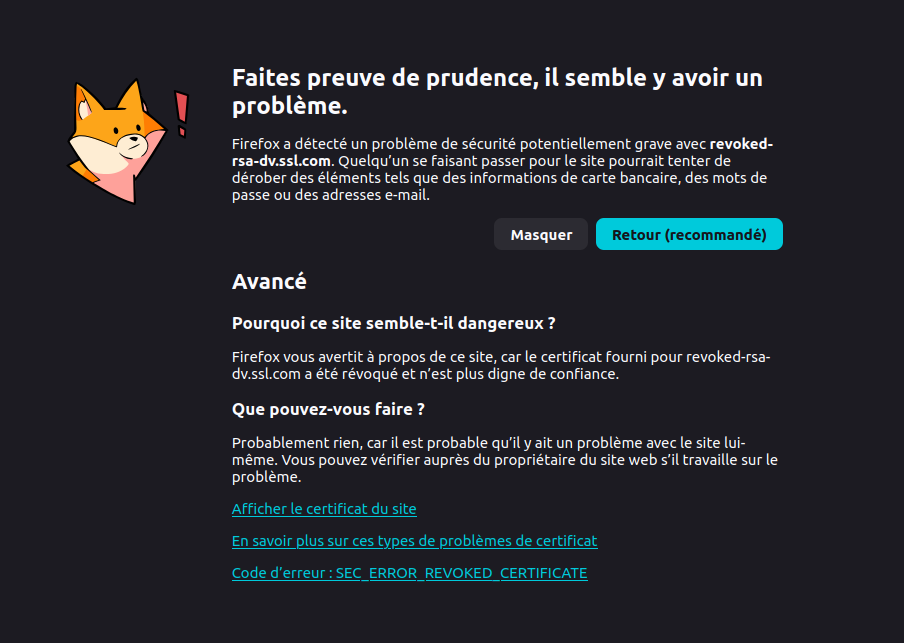
\includegraphics[width=0.48\linewidth]{figures/revoked_rsa_firefox.png}
  \caption{Blocage du certificat révoqué : erreur \file{NET::ERR_CERT_REVOKED} dans Chromium/Chrome et \file{SEC_ERROR_REVOKED_CERTIFICATE} dans Firefox.}
  \label{fig:revoked-browsers-opencode}
\end{figure}

Le certificat étudié est \file{01-public-certs/revoked-rsa-dv.ssl.com.pem}. Son numéro de série est :

\begin{lstlisting}[style=result]
1811B09C4BB9E179133BB9D9A9B140C5
\end{lstlisting}

La CRL \file{http://crls.ssl.com/SSL.com-TLS-I-RSA-R1.crl} contient bien l'entrée correspondante.

\begin{lstlisting}[style=result]
Serial Number: 1811B09C4BB9E179133BB9D9A9B140C5
Revocation Date: Jun  9 14:37:38 2026 GMT
\end{lstlisting}

\subsection{Vérification OCSP du même certificat}
\begin{lstlisting}[style=shellcmd]
openssl ocsp \
  -issuer ssl.com-tls-i-rsa-r1.pem \
  -cert revoked-rsa-dv.ssl.com.pem \
  -url http://ocsps.ssl.com \
  -no_nonce \
  -resp_text -text
\end{lstlisting}

\begin{lstlisting}[style=result]
OCSP Response Status: successful (0x0)
Cert Status: revoked
Revocation Time: Jun  9 14:37:38 2026 GMT
revoked-rsa-dv.ssl.com.pem: revoked
\end{lstlisting}

La réponse OCSP confirme la même révocation que la CRL.

\subsection{Comparaisons complémentaires}
Les certificats présentés pour \file{google.com} et \file{youtube.com} partagent le même numéro de série.

\begin{lstlisting}[style=result]
google.com  : 139CDF29A8B5BC5212413EEEAFD18CBE
youtube.com : 139CDF29A8B5BC5212413EEEAFD18CBE
\end{lstlisting}

Ils correspondent au même certificat feuille émis par \file{C=US, O=Google Trust Services, CN=WR2}, avec \file{CN=*.google.com}. Les SAN couvrent notamment \file{DNS:google.com} et \file{DNS:youtube.com}.

Pour \file{https://wrong.host.badssl.com/}, le contrôle de nom échoue comme attendu.

\begin{lstlisting}[style=result]
verify error:num=62:hostname mismatch
Verification error: hostname mismatch
\end{lstlisting}

Le nom demandé ne correspond pas aux SAN du certificat présenté; un wildcard ne couvre qu'un seul niveau de sous-domaine.

\begin{warningbox}
Aucun fichier \file{isrg-1.crt} ou \file{isrg-2.crt} n'était disponible dans l'arborescence de travail. La méthode prévue reste :
\begin{lstlisting}[style=shellcmd]
for f in isrg-1.crt isrg-2.crt; do
  openssl x509 -in $f -noout -subject -issuer -dates
  openssl x509 -in $f -noout -text | grep -E "Public Key Algorithm|Public-Key|Signature Algorithm"
done
\end{lstlisting}
\end{warningbox}

\newpage

\section{PKI OpenSSL multi-autorités}

\subsection{Organisation logique}
La hiérarchie locale reprend une structure à deux racines, l'une RSA et l'autre ECDSA. Chaque racine émet une AC subordonnée, puis ces AC émettent les certificats finaux. Une certification croisée unidirectionnelle permet à la racine RSA de valider une branche EC via un certificat supplémentaire.

\begin{center}
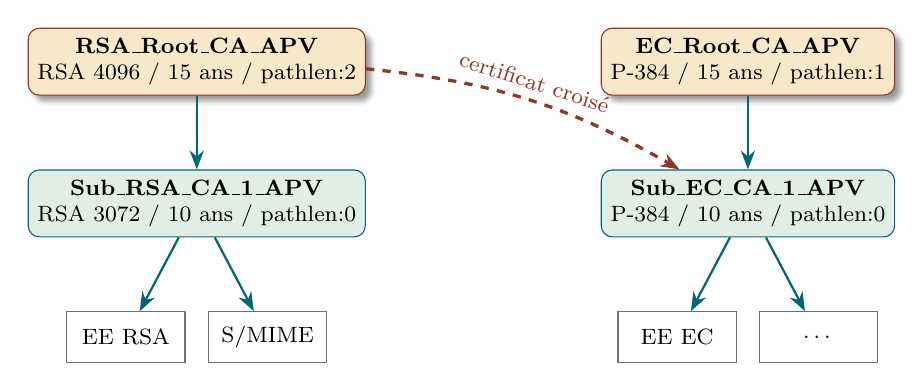
\begin{tikzpicture}[
  font=\footnotesize,
  root/.style={rectangle,rounded corners,draw=oxide,fill=sand,minimum width=3.2cm,minimum height=0.85cm,align=center,blur shadow},
  sub/.style={rectangle,rounded corners,draw=lagoon,fill=sage,minimum width=3.2cm,minimum height=0.85cm,align=center},
  leaf/.style={rectangle,draw=muted,fill=white,minimum width=1.5cm,minimum height=0.65cm,align=center},
  arr/.style={-{Stealth[length=2.4mm]},thick,lagoon},
  cross/.style={-{Stealth[length=2.4mm]},very thick,oxide,dashed}
]
\node[root] (rr) at (0,3) {\textbf{RSA\_Root\_CA\_APV}\\RSA 4096 / 15 ans / pathlen:2};
\node[root] (er) at (7,3) {\textbf{EC\_Root\_CA\_APV}\\P-384 / 15 ans / pathlen:1};
\node[sub] (sr) at (0,1.2) {\textbf{Sub\_RSA\_CA\_1\_APV}\\RSA 3072 / 10 ans / pathlen:0};
\node[sub] (se) at (7,1.2) {\textbf{Sub\_EC\_CA\_1\_APV}\\P-384 / 10 ans / pathlen:0};
\node[leaf] (r1) at (-0.9,-0.5) {EE RSA};
\node[leaf] (r2) at (0.9,-0.5) {S/MIME};
\node[leaf] (e1) at (6.1,-0.5) {EE EC};
\node[leaf] (e2) at (7.9,-0.5) {\dots};
\draw[arr] (rr) -- (sr);
\draw[arr] (er) -- (se);
\draw[arr] (sr) -- (r1);
\draw[arr] (sr) -- (r2);
\draw[arr] (se) -- (e1);
\draw[arr] (se) -- (e2);
\draw[cross] (rr) to[bend left=12] node[midway,above,sloped,oxide]{certificat croisé} (se);
\end{tikzpicture}
\end{center}

Les contraintes \file{pathLenConstraint} sont conservées : \file{pathlen:2} pour la racine RSA, \file{pathlen:1} pour la racine EC et \file{pathlen:0} pour les deux subordonnées.

\subsection{Sens unique de la certification croisée}
\begin{answerbox}
La racine \file{RSA_Root_CA_APV} signe un certificat croisé pour \file{EC_Root_CA_APV}. Un client qui fait confiance à la racine RSA peut donc reconstruire une chaîne vers la branche EC. En revanche, la branche inverse n'existe pas sans certificat miroir signé par \file{EC_Root_CA_APV} pour \file{RSA_Root_CA_APV}.
\end{answerbox}

\begin{lstlisting}[style=result]
RSA_Root_CA_APV
  -> EC_Root_CA_APV (certificat croise signe par RSA_Root_CA_APV)
  -> Sub_EC_CA_1_APV
  -> Leaf_EC_1_APV.crosspath
\end{lstlisting}

Pour rendre la relation bidirectionnelle, il faudrait émettre les deux certificats croisés suivants.

\begin{lstlisting}[style=result]
RSA_Root_CA_APV -> EC_Root_CA_APV
EC_Root_CA_APV  -> RSA_Root_CA_APV
\end{lstlisting}

\subsection{Initialisation des dossiers d'AC}
Chaque AC possède ses répertoires \file{private/} et \file{db/}. Avant toute commande \file{openssl ca}, la base, ses attributs, le compteur de série et le compteur de CRL doivent exister.

\begin{lstlisting}[style=shellcmd]
mkdir -p ca/{certs,crl,newcerts,csr,smime,ocsp}
for CA in RSA_Root_CA EC_Root_CA Sub_RSA_CA_1 Sub_EC_CA_1; do
  mkdir -p ca/$CA/db ca/$CA/private
  chmod 700 ca/$CA/private
  : > ca/$CA/db/$CA.db            # base vide mais existante
  : > ca/$CA/db/$CA.db.attr
  echo 01 > ca/$CA/db/$CA.srl     # numero de serie initial
  echo 01 > ca/$CA/db/$CA.crl.srl # numero de CRL initial
done
\end{lstlisting}

\subsection{Extrait de configuration OpenSSL}
Le passage suivant est l'extrait de configuration de la racine RSA utilisé pour les extensions racine et sous-AC.

\begin{lstlisting}[style=config]
[ca]
default_ca = root_ca

[root_ca]
certificate      = $dir/RSA_Root_CA.crt
private_key      = $dir/private/RSA_Root_CA.key
database         = $dir/db/RSA_Root_CA.db
serial           = $dir/db/RSA_Root_CA.srl
crlnumber        = $dir/db/RSA_Root_CA.crl.srl
default_md       = sha256          # hachage SHA-256 (ANSSI)
default_crl_days = 30              # CRL valable 1 mois
policy           = policy_loose

# --- profil de la racine elle-meme (auto-signature) ---
[root_ca_ext]
basicConstraints       = critical,CA:TRUE,pathlen:2   # 2 niveaux de sous-AC
keyUsage               = critical,keyCertSign,cRLSign
subjectKeyIdentifier   = hash
authorityKeyIdentifier = keyid:always

# --- profil applique aux AC subordonnees signees par la racine ---
[sub_ca_ext]
basicConstraints       = critical,CA:TRUE,pathlen:0   # ne signe que des EE
keyUsage               = critical,keyCertSign,cRLSign
crlDistributionPoints  = URI:http://crl.pki-apv.local/RSA_Root_CA.crl
authorityInfoAccess    = caIssuers;URI:http://aia.pki-apv.local/RSA_Root_CA.crt
\end{lstlisting}

La racine EC reprend le même modèle avec \file{pathlen:1}. Le fichier de la subordonnée RSA ajoute les profils d'entité finale : serveur TLS, S/MIME et OCSP.

\subsection{Émission des racines}
La racine RSA est générée puis autosignée avec une validité de 15 ans.

\begin{lstlisting}[style=shellcmd]
# 1) genere la bi-cle RSA 4096 + la CSR
openssl req -new -config ca/RSA_Root_CA/RSA_Root_CA.conf \
  -newkey rsa:4096 -keyout ca/RSA_Root_CA/private/RSA_Root_CA.key -nodes \
  -out ca/csr/RSA_Root_CA.csr
# 2) auto-signature (15 ans, extensions racine)
openssl ca -batch -config ca/RSA_Root_CA/RSA_Root_CA.conf -selfsign \
  -in ca/csr/RSA_Root_CA.csr -extensions root_ca_ext -days 5479 \
  -out ca/RSA_Root_CA/RSA_Root_CA.crt
\end{lstlisting}

\begin{lstlisting}[style=result]
$ openssl x509 -in RSA_Root_CA.crt -noout -subject -issuer -dates
subject= C = FR, O = TP IMT Mines Ales, OU = PKI APV, CN = RSA Root CA APV
issuer = C = FR, O = TP IMT Mines Ales, OU = PKI APV, CN = RSA Root CA APV
notBefore=Jun 23 06:30:04 2026 GMT
notAfter =Jun 23 06:30:04 2041 GMT          # 15 ans
    X509v3 Basic Constraints: critical
        CA:TRUE, pathlen:2
    X509v3 Key Usage: critical
        Certificate Sign, CRL Sign
\end{lstlisting}

Pour la racine ECDSA, la clé P-384 est créée explicitement avant la CSR.

\begin{lstlisting}[style=shellcmd]
# 1) cle EC P-384 (secp384r1)
openssl genpkey -algorithm EC -pkeyopt ec_paramgen_curve:secp384r1 \
  -out ca/EC_Root_CA/private/EC_Root_CA.key
# 2) CSR a partir de la cle existante
openssl req -new -config ca/EC_Root_CA/EC_Root_CA.conf \
  -key ca/EC_Root_CA/private/EC_Root_CA.key -out ca/csr/EC_Root_CA.csr
# 3) auto-signature (15 ans, pathlen:1)
openssl ca -batch -config ca/EC_Root_CA/EC_Root_CA.conf -selfsign \
  -in ca/csr/EC_Root_CA.csr -extensions root_ca_ext -days 5479 \
  -out ca/EC_Root_CA/EC_Root_CA.crt
\end{lstlisting}

\begin{lstlisting}[style=result]
$ openssl x509 -in EC_Root_CA.crt -noout -text | grep -E "Algorithm|NIST|pathlen|Sign"
        Signature Algorithm: ecdsa-with-SHA256
                ASN1 OID: secp384r1
                NIST CURVE: P-384
            CA:TRUE, pathlen:1
            Certificate Sign, CRL Sign
\end{lstlisting}

\subsection{Autorités subordonnées}
La sous-AC RSA est créée avec une clé RSA 3072 bits et signée par la racine RSA avec \file{sub_ca_ext}. Le même principe s'applique à la branche EC.

\begin{lstlisting}[style=shellcmd]
openssl req -new -config ca/Sub_RSA_CA_1/Sub_RSA_CA_1.conf \
  -newkey rsa:3072 -keyout ca/Sub_RSA_CA_1/private/Sub_RSA_CA_1.key -nodes \
  -out ca/csr/Sub_RSA_CA_1.csr
# signature par la racine RSA
openssl ca -batch -config ca/RSA_Root_CA/RSA_Root_CA.conf \
  -extensions sub_ca_ext -days 3653 \
  -in ca/csr/Sub_RSA_CA_1.csr -out ca/Sub_RSA_CA_1/Sub_RSA_CA_1.crt
\end{lstlisting}

\begin{lstlisting}[style=result]
$ openssl verify -CAfile RSA_Root_CA.crt Sub_RSA_CA_1.crt
Sub_RSA_CA_1.crt: OK
$ openssl verify -CAfile EC_Root_CA.crt  Sub_EC_CA_1.crt
Sub_EC_CA_1.crt: OK
\end{lstlisting}

\newpage

\section{Révocation, S/MIME et chemins de confiance}

\subsection{Révocation par CRL}
Le certificat \file{Sub_RSA_CA_1_APV-leaf-crl.crt} est émis dans \file{03-crl-ocsp} par \file{Sub_RSA_CA_1_APV}.

\begin{lstlisting}[style=shellcmd]
cd /home/baptiste/tp-crypto-agents/03-crl-ocsp
openssl ca -batch \
  -config openssl-rsa-sub-ocsp.cnf \
  -extensions v3_leaf \
  -days 365 \
  -notext \
  -in Sub_RSA_CA_1_APV-leaf-crl.csr.pem \
  -out Sub_RSA_CA_1_APV-leaf-crl.crt
\end{lstlisting}

La vérification de chaîne avant révocation donne :

\begin{lstlisting}[style=shellcmd]
openssl verify \
  -CAfile /home/baptiste/tp-crypto-agents/02-pki-openssl/RSA_Root_CA_APV/certs/RSA_Root_CA_APV.crt \
  -untrusted /home/baptiste/tp-crypto-agents/02-pki-openssl/Sub_RSA_CA_1_APV/certs/Sub_RSA_CA_1_APV.crt \
  Sub_RSA_CA_1_APV-leaf-crl.crt
\end{lstlisting}

\begin{lstlisting}[style=result]
/home/baptiste/tp-crypto-agents/03-crl-ocsp/Sub_RSA_CA_1_APV-leaf-crl.crt: OK
\end{lstlisting}

La révocation est ensuite publiée dans une CRL de 30 jours.

\begin{lstlisting}[style=shellcmd]
openssl ca -batch -config openssl-rsa-sub-ocsp.cnf \
  -revoke Sub_RSA_CA_1_APV-leaf-crl.crt \
  -crl_reason keyCompromise
openssl ca -config openssl-rsa-sub-ocsp.cnf \
  -gencrl -crldays 30 \
  -out ca-work/Sub_RSA_CA_1_APV/crl.pem
openssl crl -in ca-work/Sub_RSA_CA_1_APV/crl.pem -text -noout > crl-after-revoke.txt
\end{lstlisting}

\begin{lstlisting}[style=result]
Issuer: C=FR, O=TP Crypto Agents, OU=PKI OpenSSL, CN=Sub_RSA_CA_1_APV
Last Update: Jun 23 07:18:21 2026 GMT
Next Update: Jul 23 07:18:21 2026 GMT
Serial Number: 1000
Revocation Date: Jun 23 07:18:21 2026 GMT
X509v3 CRL Reason Code: Key Compromise
\end{lstlisting}

Le certificat est bien présent dans la CRL avec le motif \file{Key Compromise}.

\subsection{Certificat et échange S/MIME}
Le certificat \file{04-smime/smime-user.crt} est émis par \file{Sub_RSA_CA_1_APV}. Les extensions conservées sont \file{Basic Constraints: CA:FALSE}, \file{Key Usage: Digital Signature, Key Encipherment}, \file{Extended Key Usage: E-mail Protection} et le SAN email \file{smime-user@apv.local}.

\begin{lstlisting}[style=shellcmd]
cd /home/baptiste/tp-crypto-agents/04-smime
openssl ca -batch \
  -config ../02-pki-openssl/Sub_RSA_CA_1_APV/openssl-rsa-sub.cnf \
  -extfile smime-openssl.cnf \
  -extensions v3_smime_signer \
  -days 365 \
  -notext \
  -in smime-user.csr.pem \
  -out smime-user.crt
\end{lstlisting}

La démonstration locale utilise \file{recipient-test.crt}. L'échange réel avec un autre groupe n'est pas finalisé.

\begin{lstlisting}[style=shellcmd]
openssl smime -sign -binary -nodetach \
  -in message.txt \
  -signer smime-user.crt \
  -inkey smime-user.key.pem \
  -certfile ../02-pki-openssl/Sub_RSA_CA_1_APV/certs/Sub_RSA_CA_1_APV.crt \
| openssl smime -encrypt -aes256 \
  -out signed-encrypted-message.pem \
  recipient-test.crt

openssl smime -decrypt \
  -in signed-encrypted-message.pem \
  -recip recipient-test.crt \
  -inkey recipient-test.key.pem \
  -out decrypted-signed-message.pem

openssl smime -verify \
  -in decrypted-signed-message.pem \
  -CAfile ../02-pki-openssl/RSA_Root_CA_APV/certs/RSA_Root_CA_APV.crt \
  -out verified-message.txt
\end{lstlisting}

\begin{answerbox}
Le fichier \file{verified-message.txt} contient le message clair attendu. La chaîne locale signature, chiffrement, déchiffrement et vérification est donc validée. L'échange inter-groupe reste à réaliser.
\end{answerbox}

\begin{remarkbox}
Le sujet recommande idéalement deux certificats distincts, un pour la signature et un autre pour le chiffrement. Le TP conserve un certificat unique pour simplifier les manipulations.
\end{remarkbox}

\subsection{Répondeur OCSP local}
Le certificat testé \file{Sub_RSA_CA_1_APV-leaf-ocsp.crt} expose à la fois une URL CRL et une URL OCSP.

\begin{lstlisting}[style=result]
CRL Distribution Points:
  URI:http://crl.localhost:2560/Sub_RSA_CA_1_APV.crl
Authority Information Access:
  OCSP - URI:http://ocsp.localhost:2560
\end{lstlisting}

Le répondeur est lancé localement sur \file{127.0.0.1:2560}.

\begin{lstlisting}[style=shellcmd]
openssl ocsp \
  -index ca-work/Sub_RSA_CA_1_APV/db/index.txt \
  -port 2560 \
  -rsigner ../02-pki-openssl/Sub_RSA_CA_1_APV/certs/Sub_RSA_CA_1_APV.crt \
  -rkey ../02-pki-openssl/Sub_RSA_CA_1_APV/private/Sub_RSA_CA_1_APV.key.pem \
  -CA ../02-pki-openssl/Sub_RSA_CA_1_APV/certs/Sub_RSA_CA_1_APV.crt \
  -nrequest 1
\end{lstlisting}

Avant révocation, le statut est \file{good}.

\begin{lstlisting}[style=shellcmd]
openssl ocsp \
  -issuer ../02-pki-openssl/Sub_RSA_CA_1_APV/certs/Sub_RSA_CA_1_APV.crt \
  -cert Sub_RSA_CA_1_APV-leaf-ocsp.crt \
  -url http://127.0.0.1:2560 \
  -CAfile ../02-pki-openssl/RSA_Root_CA_APV/certs/RSA_Root_CA_APV.crt \
  -verify_other ../02-pki-openssl/Sub_RSA_CA_1_APV/certs/Sub_RSA_CA_1_APV.crt \
  -resp_text -text -no_nonce
\end{lstlisting}

\begin{lstlisting}[style=result]
Cert Status: good
Response verify OK
Sub_RSA_CA_1_APV-leaf-ocsp.crt: good
\end{lstlisting}

Après révocation, la réponse OCSP change d'état.

\begin{lstlisting}[style=shellcmd]
openssl ca -batch -config openssl-rsa-sub-ocsp.cnf \
  -revoke Sub_RSA_CA_1_APV-leaf-ocsp.crt \
  -crl_reason cessationOfOperation
\end{lstlisting}

\begin{lstlisting}[style=result]
Cert Status: revoked
Revocation Time: Jun 23 07:18:22 2026 GMT
Response verify OK
Sub_RSA_CA_1_APV-leaf-ocsp.crt: revoked
\end{lstlisting}

\subsection{Certification croisée}
L'entité finale EC destinée au test de chemin est \file{05-cross-cert/certs/Leaf_EC_1_APV.crosspath.crt}. La racine RSA signe un certificat supplémentaire pour la racine EC :

\begin{lstlisting}[style=result]
05-cross-cert/certs/EC_Root_CA_APV.cross-signed-by-RSA_Root_CA_APV.crt
\end{lstlisting}

Les deux vérifications suivantes valident d'abord le chemin natif EC, puis le chemin croisé ancré dans la racine RSA.

\begin{lstlisting}[style=shellcmd]
# Chaine native : Leaf_EC -> Sub_EC_CA_1 -> EC_Root_CA
openssl verify -show_chain \
  -CAfile /home/baptiste/tp-crypto-agents/02-pki-openssl/EC_Root_CA_APV/certs/EC_Root_CA_APV.crt \
  -untrusted /home/baptiste/tp-crypto-agents/02-pki-openssl/Sub_EC_CA_1_APV/certs/Sub_EC_CA_1_APV.crt \
  /home/baptiste/tp-crypto-agents/05-cross-cert/certs/Leaf_EC_1_APV.crosspath.crt

# Chaine croisee : Leaf_EC -> Sub_EC_CA_1 -> EC_Root_CA cross-signee -> RSA_Root_CA
openssl verify -show_chain \
  -CAfile /home/baptiste/tp-crypto-agents/02-pki-openssl/RSA_Root_CA_APV/certs/RSA_Root_CA_APV.crt \
  -untrusted /home/baptiste/tp-crypto-agents/05-cross-cert/certs/untrusted-rsa-path.pem \
  /home/baptiste/tp-crypto-agents/05-cross-cert/certs/Leaf_EC_1_APV.crosspath.crt
\end{lstlisting}

\begin{lstlisting}[style=result]
/home/baptiste/tp-crypto-agents/05-cross-cert/certs/Leaf_EC_1_APV.crosspath.crt: OK
depth=0: CN=Leaf_EC_1_APV
depth=1: CN=Sub_EC_CA_1_APV
depth=2: CN=EC_Root_CA_APV

/home/baptiste/tp-crypto-agents/05-cross-cert/certs/Leaf_EC_1_APV.crosspath.crt: OK
depth=0: CN=Leaf_EC_1_APV
depth=1: CN=Sub_EC_CA_1_APV
depth=2: CN=EC_Root_CA_APV
depth=3: CN=RSA_Root_CA_APV
\end{lstlisting}

La certification croisée reste unidirectionnelle; le miroir attendu pour une relation dans les deux sens serait \file{RSA_Root_CA_APV.cross-signed-by-EC_Root_CA_APV.crt}.

\subsection{Magasin Windows}
Cette étape n'a pas été exécutée dans l'environnement Linux. Les certificats à importer sont la racine et l'intermédiaire correspondant à la chaîne testée. Les magasins Windows visés sont \file{Cert:\LocalMachine\Root} pour la racine et \file{Cert:\LocalMachine\CA} pour l'intermédiaire.

\begin{warningbox}
Procédure préparée pour Windows Server, captures à insérer après exécution.
\begin{lstlisting}[style=shellcmd]
Import-Certificate -FilePath C:\PKI\HSM_Root_CA_APV.cer -CertStoreLocation Cert:\LocalMachine\Root
Import-Certificate -FilePath C:\PKI\HSM_Sub_CA_APV.cer  -CertStoreLocation Cert:\LocalMachine\CA
\end{lstlisting}
Validation attendue : ouverture du certificat dans Windows et contrôle de l'onglet \file{Chemin d'accès de certification}. Captures à compléter : magasin racine, magasin intermédiaire et chaîne validée.
\end{warningbox}

\newpage

\section{Racine protégée par SoftHSM2}

\subsection{Création de la racine HSM}
Sous Linux, la partie SoftHSM2 couvre la configuration du token, la génération d'une clé RSA 4096 bits non exportée, l'émission d'une racine autosignée, la génération d'une CRL/ARL mensuelle et l'utilisation d'OpenSSL via PKCS\#11.

\begin{lstlisting}[style=shellcmd]
cd /home/baptiste/tp-crypto-agents/06-softhsm
./scripts/bootstrap-hsm-root-ca.sh
\end{lstlisting}

\begin{lstlisting}[style=result]
Subject: C=FR, O=TP Crypto, OU=06-softhsm, CN=HSM_Root_CA_APV
Issuer:  C=FR, O=TP Crypto, OU=06-softhsm, CN=HSM_Root_CA_APV
Cle: RSA 4096 bits
Validite: Jun 23 07:17:04 2026 GMT -> Jun 20 07:17:04 2036 GMT
Extensions: CA:TRUE, pathlen:1, Certificate Sign, CRL Sign
\end{lstlisting}

\subsection{CRL / ARL}
\begin{lstlisting}[style=result]
Issuer: C=FR, O=TP Crypto, OU=06-softhsm, CN=HSM_Root_CA_APV
Last Update: Jun 23 07:17:04 2026 GMT
Next Update: Jul 23 07:17:04 2026 GMT
No Revoked Certificates.
\end{lstlisting}

\subsection{Contrôle d'absence de clé privée exportée}
\begin{lstlisting}[style=shellcmd]
sh scripts/verify-no-private-files.sh
\end{lstlisting}

\begin{lstlisting}[style=result]
No private key file (.key or private .pem) found outside SoftHSM2.
\end{lstlisting}

\begin{remarkbox}
Aucun PIN, mot de passe, secret de token ou contenu de clé privée n'est reproduit dans ce rapport. Les commandes nécessitant un PIN doivent passer par une variable d'environnement locale ou par une saisie interactive.
\end{remarkbox}

\subsection{Note PKCS\#11 et ADCS}
La tentative avec le provider \file{pkcs11} a échoué car le module attendu n'existait pas sous ce nom. La solution retenue est le provider OpenSSL 3 \file{pkcs11prov}, avec le module SoftHSM2 configuré.

La partie ADCS doit être exécutée sur Windows Server 2019. Le dossier \file{07-windows-handoff/README.md} documente la préparation, sans preuve d'exécution finale.

\begin{warningbox}
Procédure attendue pour l'AC subordonnée Windows et le certificat TLS associé.
\begin{enumerate}[leftmargin=1.5em]
  \item Installer ADCS en mode \emph{Standalone CA} :
\end{enumerate}
\begin{lstlisting}[style=shellcmd]
Install-WindowsFeature ADCS-Cert-Authority -IncludeManagementTools
\end{lstlisting}
\begin{enumerate}[leftmargin=1.5em,resume]
  \item Créer une AC subordonnée autonome avec clé RSA 4096 bits, SHA-256 et validité 5 ans :
\end{enumerate}
\begin{lstlisting}[style=shellcmd]
Install-AdcsCertificationAuthority `
  -CAType StandaloneSubordinateCA `
  -CACommonName "HSM_Sub_CA_APV" `
  -KeyLength 4096 `
  -HashAlgorithmName SHA256 `
  -CryptoProviderName "RSA#Microsoft Software Key Storage Provider" `
  -OutputCertRequestFile C:\PKI\HSM_Sub_CA_APV.req `
  -ValidityPeriod Years `
  -ValidityPeriodUnits 5
\end{lstlisting}
\begin{enumerate}[leftmargin=1.5em,resume]
  \item Transférer la CSR PKCS\#10 vers Linux et la signer avec la racine OpenSSL/SoftHSM2 :
\end{enumerate}
\begin{lstlisting}[style=shellcmd]
cd /home/baptiste/tp-crypto-agents/06-softhsm
./scripts/sign-adcs-csr.sh HSM_Sub_CA_APV.req issued/HSM_Sub_CA_APV.crt
\end{lstlisting}
\begin{enumerate}[leftmargin=1.5em,resume]
  \item Renvoyer le certificat signé sur Windows et finaliser ADCS :
\end{enumerate}
\begin{lstlisting}[style=shellcmd]
certreq -accept C:\PKI\HSM_Sub_CA_APV.cer
\end{lstlisting}
\begin{enumerate}[leftmargin=1.5em,resume]
  \item Générer une requête TLS avec \file{certreq}, puis la soumettre à l'AC ADCS :
\end{enumerate}
\begin{lstlisting}[style=shellcmd]
certreq -new C:\PKI\tls.inf C:\PKI\tls.req
certutil -config "NomServeur\HSM_Sub_CA_APV" -submit C:\PKI\tls.req C:\PKI\tls.cer
\end{lstlisting}
Captures nécessaires : rôle ADCS installé, AC subordonnée configurée, certificat racine importé, certificat subordonné valide, certificat TLS émis et chaîne visible dans Windows.
\end{warningbox}

\end{document}
